\chapter{Analysing the Models}\label{ana_models}
In this chapter, we will study how to properly perform tests on NNs to measure and analyse their characteristics and to find links among them in the context of the recognition of sugar beets. Although it is possible to predict some of the characteristics using NNs’ weights (\cite{Unterthiner2020PredictingNN}), in this paper we will rely upon methods to find them empirically. The output of our investigation will be a toolbox which we can easily run on most devices to measure the characteristics we are mostly interested in. \\
In section \ref{benchmarking} e will explore the concept of benchmarking in general terms to make an idea of the requirements we will need to full-fill to produce reliable results. In section \ref{benchmarking_nn} we will dive deep into measuring NNs' performances and we will introduce techniques we can use for our own benchmark. Finally, in section \ref{sec:my_bench} we will describe the benchmark to use it in future sections to measure the characteristics of some networks. 

\section{Benchmarking}\label{benchmarking}
Benchmarking is a widely used tool to evaluate the performance of a system, either software or hardware, whose main goal is to produce consistent and precise measurements of said systems. High precision and reliability in benchmarks, however, have been always tricky to achieve and the complexity of these tasks have reached a high complexity in recent years, due to advanced processor designs and very intricate interaction between programs and operating systems. \cite{DBLP:journals/corr/abs-1811-01412}\\
In addition, knowledge about the timing behaviour of tasks, more specifically their worst- case execution times (WCETs), is of the highest importance for building reliable and dependable real-time systems.\cite{Real-Time-Systems}\\
According to \textit{von Kistowski et al.} in \cite{how_to_bench}, benchmarks should follow certain key characteristics in order to be reliable:

\begin{itemize}
    \item Relevance
    \item Reproducibility
    \item Fairness
    \item Verifiability
    \item Usability
\end{itemize}
%In the next section, we will better define them and describe them thoroughly. Understanding these characteristics is essential to produce precise and reliable measurements. Subsequently, we will explore some common techniques used to benchmark software. In section \ref{sec:remove_inter}, some of the main roadblocks and pitfalls of benchmarks are described to help the reader avoid them. In the same section, we will also point out some strategies to reduce measurement noise. Finally, in section \ref{sec:my_bench}, the benchmark used in this paper is described to facilitate its reproducibility. \\









\subsection{Key Characteristics for a Correct Benchmark}\label{key_char}
%In this section, we will explore the main characteristics a benchmark should possess in order to be a regarded as a reliable benchmark.
\subsubsection{Relevance}
Relevance is probably the most important criteria for benchmarks. Relevance measures how close the behavior of the benchmark relates to the behaviors it is trying to test. \cite{how_to_bench}\\
Even if the benchmark is realized perfectly and respects all the other characteristics, if the results do not provide relevant information they are of no use. It is when the relevance of the benchmark is taken into account that the computer scientists or engineers need to make the first trade-offs and the first considerations. As a matter of fact, benchmarks that are designed to be highly relevant in a specific scenario tend to have a narrow applicability; vice-versa, benchmarks with a broader spectrum are usually less indicative in specific scenarios. \cite{how_to_bench}\\
Relevance also relates to the scalability of the benchmark. For example, benchmarks designed to test the full ability of servers might use the full resources that the server offers, for e.g. multi-threading, and as such it will not perform correctly in systems that do not have this possibility. \cite{how_to_bench}

\subsubsection{Reproducibility}
Reproducibility is the ability to consistently obtain similar, if not equivalent, results if the benchmark is tested on the same environment. \cite{how_to_bench}\\
Reproducibility is tightly correlated to the ability of describing the environment in perfect detail, so that it could be performed on the same environment and expect similar results. The hardware must be described perfectly and software versions must be included and documented, as well as every other configuration done on the system. Especially with the increase of complexity in modern hardware architecture and modern operating systems, variability in performance is introduced by several factors, including timing of thread scheduling, physical disk layout and user interaction. \cite{how_to_bench}\\
Such variability can be addressed by running the benchmark for long enough periods of time in steady state, therefore without factors like user interaction.


\subsubsection{Fairness}
In order to create a perfect benchmark, fairness is a characteristic that should be taken into account. A fair benchmark is a benchmark that allows the results obtained in different systems with completely different hardware and software to be comparable. Benchmarks are simplistic and, by their very nature, include a certain degree of artificiality, so it is necessary to put some constraints in order to stop the programs to ”exploit” them. Those restrictions can be put, for example, in the software used.\\ 
\textit{Kistowski et al.} in \cite{how_to_bench} pointed out, for example, a benchmark realized in Java requires a virtual machine on top of the operating systems and the choice of virtual machine can heavily influence the results. This shows how limiting software and hardware components must be carefully limited to ensure fairness in the results. However, putting too many limitations may actually hide some of the results, which might be relevant (\cite{how_to_bench}). Therefore it is essential to find a good balance amongst the different limitations. Furthermore, portability plays a huge role in a fair benchmark. If too many limitations are imposed, or if those limitations are too strict, a big pool of devices could be not suitable to run the benchmark. Similarly to the amount of limitations, portability is also a factor which requires a trade off. As a matter of fact, the portability of a benchmark strictly depends on the very nature of the devices which are set to be used.

\subsubsection{Verifiability}
A good benchmark should be able to provide trustworthy results and also results whose trustworthiness can be verified. To ensure the verifiability of the results, good benchmarks usually run some self-verification tasks during run-time, for e.g. if hyper-threading is still active when it should not. Moreover, it is also the case that some benchmarks let users configure some parameters. Those configurations should be documented, as an undocumented alteration might define the result as not trustworthy. \cite{how_to_bench}\\
Finally, it is also good practice to include more metrics in the results other than the ones strictly needed, since some red flags might be raised by inconsistencies in these metrics.
\subsubsection{Usability}
Usability is the characteristics of a benchmark which aims to remove roadblocks for users to run the benchmark in their environments. This feature is not limited to how easy it is to run the benchmark, which should be not a complex task, but some of the aforementioned characteristics relate to this one. For example, a good description of the benchmark also improves the usability of it, since it is easier to replicate. In addition, if the benchmark is too complex or expensive for its purpose it might limit a potential user and not allow them to effectively reproduce the tests.



\subsection{Benchmark Techniques and Methodologies}\label{BTaM}

This section will delineate the different methodologies to measure the execution time of programs. It will contain techniques for both the \textit{wall time} and the \textit{CPU time}. \\
We are going to use the term  \textit{CPU time} to define the time spent by the CPU to process a piece of software, while we are going to use the term \textit{Wall Time} to indicate the time elapsed between the start and the end of the execution of a program.\\\hfill
Measuring the wall time of a program is the most straightforward, as it can also be done analogically using a manual stopwatch: simply start the time as the program starts and stop it as the program finishes. This method is undoubtedly imprecise and not very flexible, as it can only be applied to program whose needed measurements are just rough approximation. \cite{Stewart2001MeasuringET}\\
The equivalent method in UNIX-like systems is by using the command \textit{date}, which returns the system date and time. Due to the imprecise nature of such a method it will not be described further. \\
A method along the lines of the one described above is by using functions like \textit{clock()} within the program we are trying to benchmark. This function needs to be used within the code of the program, similarly to the snippet of code in Fig n.\ref{fig:code} (\cite{Stewart2001MeasuringET}), therefore it is limited to measure only small parts of the program. \\
\begin{figure}
\begin{lstlisting}[language=C, label= code]
    #include <time.h>
    
    //...
    
    clock_t start,finish;
    double total;
    start = clock();
    // Insert function here
    finish = clock();
    total = (double) (finish - start) / (double) CLK_TCK
    printf("Total = %f\n",total);
    
\end{lstlisting}
\caption{This snippet of code shows an example of use of the function \textit{clock()}}
\label{fig:code}
\end{figure}
In addition, such functions present two other problems. Since the function does not have a standardized implementation, the result may vary from device to device, which makes reproducibility impossible. Furthermore, this type of functions needs to be executed as well, similarly to any other function in the code, hence they might introduce overhead and noise in the measurements.\\

A better way to measure the \textit{wall time} of a program is to use the UNIX command \textit{time}. The synopsis for this program is the following (\cite{linux_commands}):\\
\begin{figure*}[h]
\begin{lstlisting}[language=bash]
   $ time [options] command [arguments...]
\end{lstlisting}
\caption{Synopsis of the command \textit{time}}
\label{fig:time_code}
\end{figure*}


The \textit{time} command runs the specified \textbf{command}, which can be running a specific program, and, as the program finishes, it returns the timing statistics about this program run.
These statistic consist of \textit{(i)} the elapsed real time between start and end of the program, hence the wall time, defined as \textbf{real}; \textit{(ii)} the CPU time, excluding I/O blocking functions, time for preemption and the time used for other OS related functions, defined as \textbf{user}, or user time;\textit{(iii)} and the time spent by the OS to execute tasks on behalf of the user, defined as \textbf{sys}, or system time. The last one includes time for preemption and I/O blocking functions, or any other function associated with the program. \cite{Stewart2001MeasuringET}
It is worth to note that some shells have a built-in \textit{time} command, hence may vary from the original one. To access the real one, it is suggested to specify its path-name (for i.g. /usr/bin/time). \cite{linux_commands} 

Nevertheless, we can run a small C++ program to give an example of how to use this command and to analyze its output. The snippet of the code can be seen in Fig. \ref{fig:time_code_cpp}. The program we are going to use simply accumulates numbers from 0 to 10000000000 and prints the result on screen. Before we start accumulating, however, we add a small delay, namely 1 second, to check if this will be counted in the CPU time. Once the code has been compiled, we can run it as shown in Fig. \ref{fig:time_code}, hence by writing \textit{''time ./accumulate''} in the shell \footnote{''accumulate'' is the name of the program and we assume to be in the correct directory}.\\
From the result we can observe the three indications of time we described earlier (user, system and total time).  In the case of the machine used for this paper, the user time was roughly 24,11 seconds, the system time roughly 0,05 seconds and the total time 25,254 seconds. \\
From these measurements, we can clearly observe that the total time is around one second bigger than the user time and the system time combined and it is due to the delay we introduced in line 6. If we comment out this line and we run the test once again, the total time now roughly equalizes the combination of user and system time (23,46s user 0,03s system, 23,578 total)


\begin{figure*}[h]
\begin{lstlisting}[language=c]
    #include <iostream>
    #include <chrono>
    #include <thread>
    
    int main(){
        std::this_thread::sleep_for(std::chrono::milliseconds(1000));
        double accumulate = 0 ;
        for(double i= 0; i< 10000000000; i++)
            accumulate += i;
        std::cout << "Result : "<< accumulate <<std::endl;  
        return 0;
    }
\end{lstlisting}
\caption{Program used to test the command \textit{time}}
\label{fig:time_code_cpp}
\end{figure*}


Even though the \textit{time} command offers varied information, the time calculated and shown might not be fully reliable. As pointed out by \textit{Beyer et al.} in \cite{Beyer2017ReliableBR}, this command does not reliably include the CPU time of child processes. This is due to the fact that the Linux kernel is able to count the CPU time of a child process if that process terminated before the parent and the parent waited for it. If this happens, the CPU time of the child is lost and this will interfere with the precision of the measurements.\cite{Beyer2017ReliableBR}\\ \hfill

\textit{Beyer et al.} in \cite{Beyer2017ReliableBR} introduces yet another tool for benchmarks in their solution: control groups (cgroups). The Linux manual defines cgroups as \textit{''a Linux kernel feature which allows processes to be organized into hierarchical groups whose usage of various types of resources can then be limited and monitored''} \cite{LinuxManualWeb}. Cgroups therefore allow the user to assign processes to a group and every child process spawned by the assigned process will be tracked down. \\
Cgroups were initially released with Linux 2.6.24, however, due to the problems with the initial version, starting from Linux 3.10, cgroups version2 has been introduced. In this paper, we will not describe the differences between the two versions, as it is not the purpose of this paper (we refer to the Linux manual for further details \footnote{ \url{https://man7.org/linux/man-pages/man7/cgroups.7.html}}) and the \textit{controllers} we are interested in did not change in functionality.  \textit{Controllers} allow the user to easily control and measure a specific resource within each group. \cite{Beyer2017ReliableBR}\\
The following \textit{controllers} are the ones we are most interested in:
\begin{itemize}
    \item[] \textbf{cpu} \quad    can guarantee a minimum number of CPU resources, even when the system is busy. However, this does not limit the CPU use in case of a free CPU
    \item[] \textbf{cpuacct} \quad provides information about the accumulated CPU usage
    \item[] \textbf{cpuset} \quad restricts the number of CPU cores available to a cgroup. In a system with more than one CPU and nonuniform memory access (NUMA) it allows to restrict also the process to a subset of the physical memory  \cite{Beyer2017ReliableBR}
    \item[] \textbf{freezer} \quad allows to suspend and resume all processes in the group
    \item[] \textbf{pids} \quad allow to limit the number of spawnable processes. 
\end{itemize}
In addition to a more precise calculation of the CPU time, \textit{cgroups} also augment the fairness and the verifiability of the benchmark. By limiting the resources of a more powerful machine, the benchmark can have similar results to a much less powerful one, hence increasing fairness. 
Although this approach may hinder usability, as it is more cumbersome to set up than using the \textit{time} command, the benefits in precision make up for this trade-off. 
\subsection{Common Practices in Benchmarking}\label{sec:ben_challenges} \label{sec:remove_inter}
In section \ref{BTaM}, we already discussed some of the issues which can be encountered when trying to design benchmarks. The pitfalls, however, are not limited to those challenges; on the contrary, it is notoriously difficult to obtain consistent results when designing benchmarks. In this section, we will explore some techniques to effectively reduce the non-determinism of lots of features, both hardware and software, which intend to increase performances. In most cases, since we have little to no control over them, the solution will be to disable those features. Although it will effectively get rid of the non-determinism, the environment we are going to create does not reflect how the application will run on a real application, however it would allow us to obtain consistent results. \\
The first element we are going to analyse is Turbo-boost. This feature will automatically make the processor core run faster than the marked frequency. \textit{Acun et al.} in \cite{turbo_boost} calculated an execution time difference of up to 16\% amongst processors on the Turbo Boost-enabled supercomputers. Since we have little control over it, the only solution to limit this variation is to completely disable it. The commands to permanently disable it are shown in Fig. \ref{fig:no_boos}
\begin{figure}[h]
\begin{lstlisting}[language=bash]
# Intel
echo 1 > /sys/devices/system/cpu/intel_pstate/no_turbo
# AMD
echo 0 > /sys/devices/system/cpu/cpufreq/boost
\end{lstlisting}
\caption{Command to disable turbo boost in both AMD and Intel devices}
\label{fig:no_boos}
\end{figure}

Modern CPUs often employ a technique called Simultaneous multi-threading (SMT) to speed up execution. This technique makes it possible for two threads to run simultaneously on the same core sharing execution resources like the cache or ALU. In the case of Intel processor, the implementation of this technology is called Hyper-threading.\\
As a result of this implementation, it might occur that the sibling thread steals cache space, for example, from the workload we want to measure. To avoid these situations and limit the number of CPU-migrations, we will need to disable Hyper-threading by turning down the sibling thread in each core as shown in Fig. \ref{fig:no_ht}. 
\begin{figure}[h]
\begin{lstlisting}[language=bash]
# X being the CPU number
echo 0 > /sys/devices/system/cpu/cpuX/online
# To check the pair of CPU x
/sys/devices/system/cpu/cpuX/topology/thread_siblings_list
\end{lstlisting}
\caption{Command to disable Hyper-Threading}
\label{fig:no_ht}
\end{figure}

Another technique we can use to reduce noise in our measurements is to bind a process to a certain CPU core. In Linux we can do that with the \textit{taskset} tool. \cite{LinuxManualWeb}\\
Furthermore, we can increase the process priority with the command \textit{nice}. Processes with higher priority will get more CPU time since the Linux scheduler will favour them compared to processes with normal priority of 10. \cite{LinuxManualWeb}\\
A further step to take is to set the scaling governor policy to be \textit{performance}. The scaling governor changes the clock speed of the CPUs on the fly to save battery power, because the lower the clock speed, the less power the CPU consumes. To set the policy to be \textit{performance} one can use the method described in Fig. \ref{fig:per_sca}
\begin{figure}[h]
\begin{lstlisting}[language=bash]
for i in /sys/devices/system/cpu/cpu*/cpufreq/scaling_governor
do
  echo performance > $i
done
\end{lstlisting}
\caption{Command to set the scaling governor policy to be \textit{performance} for every CPU}
\label{fig:per_sca}
\end{figure}



\section{Benchmarking Deep Neural Networks}\label{benchmarking_nn}
Now that we have understood benchmarks and the characteristics they should possess, we can explore in greater depth how we can benchmark Deep Neural Network (DNN).\\
As expressed by \textit{Reddi et al. } in \cite{reddi2020mlperf}, ''Designing ML benchmarks is different from designing traditional non-ML benchmarks''. As a matter of fact, the spectrum of tasks NNs can perform is very broad, consequently there is a wide spectrum of requirements they need to fulfil, making the development of a reliable and relevant benchmark, which is at the same time universal, untreatable. Additionally, in this paper, we are interested in measuring performances in image classification tasks in the settings of sugar beet recognition. And although benchmarks are usually designed to compare performances, the scope of our investigation is to precisely measure the characteristics of Neural Networks and to find possible correlations amongst them.



\subsection{Benchmark Inference Time}\label{sec:ben_inf}
As we have already delineated in section n. \ref{sec:inference_time_definition}, inference time is one essential characteristic of DNN and in some cases fast inference time is an important requirement, therefore speeding up calculations is of vital importance. To achieve faster inference time, and faster calculations in general, DNNs are trained and run on Graphics processing units (GPUs), which means exploiting their hardware acceleration capabilities and their asynchronous execution (multi-threading).  (\cite{8090194}, \cite{10.1007/978-3-642-04274-4_39}, \cite{10.1145/3089801.3089804}, \cite{paine2013gpu}, \cite{OH20041311})\\
In order to measure inference time, we can apply the watchdog approach we discussed earlier in section \ref{BTaM} as shown in Fig. \ref{fig:wrong_inf}. As we already stated in the previous section, multi-threading is a factor which must be taken into account when performing benchmarking, since it could be a source of indeterminism. To prevent that, in the snippet of code in Fig. \ref{fig:wrong_inf}, taken from the benchmark developed by \textit{Bianco et al.} in \cite{bianco2018dnnsbench}, there is a call to the function \textit{torch.cuda.synchronize()}. This function is used to synchronise the host and the device, i.e. GPU and CPU, so the time is recorded only once the processes running on the GPU are terminated. Although overcoming arguably one of the biggest issues, further inspection of the code reveals some potential errors.\\
\begin{figure}[h]
\begin{lstlisting}[language=python]
def measure(model, x):

   # synchronize gpu time and measure fp
	torch.cuda.synchronize()
	t0 = time.time()
	with torch.no_grad():
		y_pred = model(x)
	torch.cuda.synchronize()
	elapsed_fp = time.time() - t0
	
	return elapsed_fp

\end{lstlisting}
\caption[Imprecise way to benchmark for inference time]{Imprecise way to benchmark for inference time \cite{bianco2018dnnsbench}}
\label{fig:wrong_inf}
\end{figure}




Although the function \textit{time.time()} is insinuated to be better and more accurate than the UNIX equivalent in the python documentation\footnote{ \url{https://docs.python.org/3/library/time.html\# time.time} }, it calculates the CPU time, hence it is not accurate if the model is run on a GPU. One way to prevent this is to use a CUDA event. Pytorch provides a useful wrapper class for them, namely \textit{torch.cuda.Event}\footnote{ \url{https://pytorch.org/docs/stable/generated/torch.cuda.Event.html} }. Moreover, GPU initialization must be taken into account as well. When the GPU is not used, it enters a lower power state in which the GPU shuts down parts of the hardware. In this state, any program which invokes the GPU will cause the drive to load anew, or the GPU to initialise once again, processes which might need a significant amount of time. It is therefore necessary to run the model some times - before measuring inference time. \cite{Correct_inference_measure}
Finally, one must be careful with transferring data between the CPU and GPU. This is usually done accidentally, when the tensor is created on the CPU and then run on the GPU. This memory allocation process takes a considerable amount of time which will influence the measurements. \cite{Correct_inference_measure}
With these corrections, a more correct measurement for inference can be found with the snippet of code in Fig. \ref{fig:corr_inf}.\\
\begin{figure}[h]
\begin{lstlisting}[language=python]
def measure(model, x):
   device = torch.device("cuda")
    model.to(device)
    dummy_input = torch.randn(1, 3,224,224, dtype=torch.float).to(device)
    start = torch.cuda.Event(enable_timing=True)
    end =  torch.cuda.Event(enable_timing=True)
    timings=np.zeros((repetitions,1))
    #GPU WARM UP
    for _ in range(10):
        _ = model(dummy_input)
    # MEASURE PERFORMANCE
    with torch.no_grad():
    for rep in range(300):
        start.record()
        _ = model(dummy_input)
        end.record()
        torch.cuda.synchronize()
        timings[rep] = start.elapsed_time(end)
    mean_syn = np.sum(timings) / repetitions
    std_syn = np.std(timings)
    print(mean_syn)

\end{lstlisting}
\caption{More precise way to measure inference time}
\label{fig:corr_inf}
\end{figure}

For the purpose of this paper, we are, purposely, going to mainly explore techniques which can be applied to Unix-like operating systems. However, there are techniques which can be applied to other types of devices, as well. For example, in case the models need to be run on a mobile device, Tensorflow Lite provides benchmarking tools to measure inference time, both in warming up and steady state. \cite{tensorflow2015-whitepaper}\\ 
For Android device, the benchmark can be run the command shown in Fig. \ref{fig:bench_ten_lite_an}.\\


\begin{figure}[h]
\begin{lstlisting}[language=bash]
adb shell am start -S \
  -n org.tensorflow.lite.benchmark/.BenchmarkModelActivity \
  --es args '"--graph=/data/local/tmp/your_model.tflite \
              --num_threads=4"'
\end{lstlisting}
\caption[Method to benchmark on Android with Tensorflow Lite]{Method to benchmark on Android with Tensorflow Lite \cite{tensorflow2015-whitepaper}}
\label{fig:bench_ten_lite_an}
\end{figure}


The result of this command is a log file which can be accessed by the command shown in Fig.\ref{fig:inf_ten}.\\
\begin{figure}[h]
\begin{lstlisting}[language=bash]
adb logcat | grep "Average inference"
\end{lstlisting}
\caption[Command to access the measured inference time in Tensorflow-Lite]{Command to access the measured inference time in Tensorflow-Lite \cite{tensorflow2015-whitepaper}}
\label{fig:inf_ten}
\end{figure}



Finally, since this paper is mainly focused on detection sugar beet plants from images, and since Convolutional Neural Networks (CNNs) became dominant for image recognition tasks (\cite{articleCNN}), it is also worth mentioning that inference time for this class of Neural Networks can be calculated manually, knowing the architecture of the model. Inference time is the time the model needs to forward propagating the image through each layer, therefore is the amount of computations needed to be performed at each of the steps. These operations are defined as Floating Point Operation, or FLOP. The amount of FLOPs is different for each layer and requires different information to be computed. \\
In case of the convolutions layers, the number of flops is calculated with the following equation:
\begin{equation}
C\_FLOPs = 2\times Nk \times Ks \times Os
\end{equation}
where:
\begin{itemize}
\item[] Nk - number of kernels
\item[] Ks - kernel shape (3x3,5x5, 7x7, etc.)
\item[] Os - Output shape
\end{itemize}
For the fully connected layers, the amount of FLOPs is defined as:
\begin{equation}
FCL\_FLOPs = 2\times Is \times OS
\end{equation}
where:
\begin{itemize}
\item[] Is - Output shape
\item[] Os - Output shape
\end{itemize}
For the pooling layer, the number of FLOPs also depends whether there is a stride or not. In case of a stride-less pooling layer, the formula to use is the following:
\begin{equation}
PL\_FLOPs = H \times D \times W
\label{eq:Pl_FLOPS}
\end{equation}
where:
\begin{itemize}
\item[] H - height of the image
\item[] D - depth of the image
\item[] W - width of the image
\end{itemize}
In case of a stride, equation n.\ref{eq:Pl_FLOPS} becomes:
\begin{equation}
PL\_FLOPs = (H/S) \times D \times (W/S)
\end{equation}
where:
\begin{itemize}
\item[] S - stride
\end{itemize}

To better understand the use of the aforementioned equations, we can calculate the FLOPs of the neural network described in Fig.\ref{fig:example-convolutional-network}. 

\usetikzlibrary{decorations.pathreplacing}
\begin{figure}[th!]
	\centering
	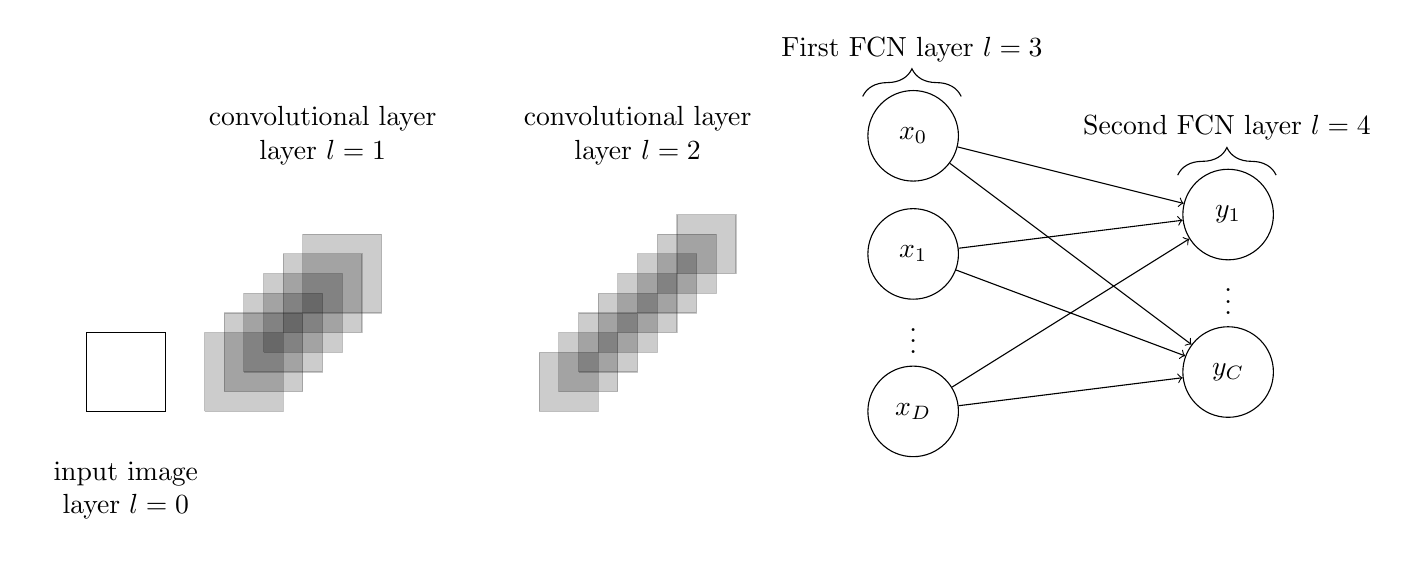
\begin{tikzpicture}
		\node at (0.5,-1){\begin{tabular}{c}input image\\layer $l = 0$\end{tabular}};
		
		\draw (0,0) -- (1,0) -- (1,1) -- (0,1) -- (0,0);
		
		\node at (3,3.5){\begin{tabular}{c}convolutional layer\\layer $l = 1$\end{tabular}};
		
		\draw[fill=black,opacity=0.2,draw=black] (2.75,1.25) -- (3.75,1.25) -- (3.75,2.25) -- (2.75,2.25) -- (2.75,1.25);
		\draw[fill=black,opacity=0.2,draw=black] (2.5,1) -- (3.5,1) -- (3.5,2) -- (2.5,2) -- (2.5,1);
		\draw[fill=black,opacity=0.2,draw=black] (2.25,0.75) -- (3.25,0.75) -- (3.25,1.75) -- (2.25,1.75) -- (2.25,0.75);
		\draw[fill=black,opacity=0.2,draw=black] (2,0.5) -- (3,0.5) -- (3,1.5) -- (2,1.5) -- (2,0.5);
		\draw[fill=black,opacity=0.2,draw=black] (1.75,0.25) -- (2.75,0.25) -- (2.75,1.25) -- (1.75,1.25) -- (1.75,0.25);
		\draw[fill=black,opacity=0.2,draw=black] (1.5,0) -- (2.5,0) -- (2.5,1) -- (1.5,1) -- (1.5,0);
		
		\node at (7,3.5){\begin{tabular}{c}convolutional layer\\layer $l = 2$\end{tabular}};
		
		\draw[fill=black,opacity=0.2,draw=black] (7.5,1.75) -- (8.25,1.75) -- (8.25,2.5) -- (7.5,2.5) -- (7.5,1.75);
		\draw[fill=black,opacity=0.2,draw=black] (7.25,1.5) -- (8,1.5) -- (8,2.25) -- (7.25,2.25) -- (7.25,1.5);
		\draw[fill=black,opacity=0.2,draw=black] (7,1.25) -- (7.75,1.25) -- (7.75,2) -- (7,2) -- (7,1.25);
		\draw[fill=black,opacity=0.2,draw=black] (6.75,1) -- (7.5,1) -- (7.5,1.75) -- (6.75,1.75) -- (6.75,1);
		\draw[fill=black,opacity=0.2,draw=black] (6.5,0.75) -- (7.25,0.75) -- (7.25,1.5) -- (6.5,1.5) -- (6.5,0.75);
		\draw[fill=black,opacity=0.2,draw=black] (6.25,0.5) -- (7,0.5) -- (7,1.25) -- (6.25,1.25) -- (6.25,0.5);
		\draw[fill=black,opacity=0.2,draw=black] (6,0.25) -- (6.75,0.25) -- (6.75,1) -- (6,1) -- (6,0.25);
		\draw[fill=black,opacity=0.2,draw=black] (5.75,0) -- (6.5,0) -- (6.5,0.75) -- (5.75,0.75) -- (5.75,0);


		\tikzstyle{unit}=[draw,shape=circle,minimum size=1.15cm]
 
        \node[unit](x0) at (10.5,3.5){$x_0$};
        \node[unit](x1) at (10.5,2){$x_1$};
        \node(dots) at (10.5,1){\vdots};
        \node[unit](xd) at (10.5,0){$x_D$};
 
        \node[unit](y1) at (14.5,2.5){$y_1$};
        \node(dots) at (14.5,1.5){\vdots};
        \node[unit](yc) at (14.5,0.5){$y_C$};
 
        \draw[->] (x0) -- (y1);
        \draw[->] (x0) -- (yc);
 
        \draw[->] (x1) -- (y1);
        \draw[->] (x1) -- (yc);
 
        \draw[->] (xd) -- (y1);
        \draw[->] (xd) -- (yc);
 
        \draw [decorate,decoration={brace,amplitude=10pt},xshift=-4pt,yshift=0pt] (10,4) -- (11.25,4) node [black,midway,yshift=+0.6cm]{First FCN layer $l = 3$};
        \draw [decorate,decoration={brace,amplitude=10pt},xshift=-4pt,yshift=0pt] (14,3) -- (15.25,3) node [black,midway,yshift=+0.6cm]{Second FCN layer $l = 4$};
	\end{tikzpicture}
	\caption[Architecture of the convolutional neural network used as an example to calculate inference time]{ Architecture of the convolutional neural network used as an example to calculate inference time. Layer $l=0$ is the input layer, with dimension $28\times 28\times 1$; $l= 1$ is the first convolution layer with a kernel of 3x3x5 and an output shape of $26\times 26\times 5$; $l=2$ is the second convolution layer with a kernel of $3\times 3\times 5$ and an output shape of $24\times 24\times 5$;$l=3$ is the first fully connected layer (FCN) with an input size of $24\times 24\times 5$ and an output size of $128$;$l=4$ is the second FCN, and final layer, with an input size of $128$ and an output size of $10$ }
	\label{fig:example-convolutional-network}
\end{figure}
The total number of FLOPs is given by:
\begin{equation}
    \begin{aligned}
&First Convolution - 2x5x(3x3)x26x26 = 60,840 FLOPs \\
&Second Convolution -2x5x(3x3x5)x24x24 = 259,200 FLOPs \\
&First FC Layer - 2x(24x24x5)x128 = 737,280 FLOPs \\
&Second FC Layer - 2x128x10 = 2,560 FLOPs\\
&FLOPs = 60,840 + 259,200 + 737,280 + 2,560 = 1,060,400 
    \end{aligned}
\end{equation}

Supposing that the processor used performs at 1 Giga FLOPS ( Floating Point Operations per Second), the inference time is given by:
\begin{equation}
    \begin{aligned}
InferenceTime &= \dfrac{FLOPs}{FLOPS} \\
          &= \dfrac{1,060,400}{1,000,000,000}\\
          &= 0.0010604\\
          &= 1,0604 ms
    \end{aligned}
    \label{eq:inference_theor}
\end{equation}
Equation n.\ref{eq:inference_theor}, however, only reveals a theoretical, ideal, value for inference time. As a matter of fact, even though the number of FLOPs remains constant, the amount of FLOPs in a processor might not.The number of FLOPs is calculated as :
\begin{equation}
FLOPS = Number\_of\_Cores \times Average\_frequency \times Operations\_per\_cycle
\end{equation}
Although the number of cores is an easy-to-find and a stable value, the average frequency and operations per cycle are not. The operating frequency is usually a lower bound of the actual operating frequency and in modern processors may vary drastically due to technologies such as TurboBoost(Intel) or Turbo Core(AMD). For example, a modern Intel\textregistered Core\textsuperscript{TM}  i7-4500U Processor has a base frequency of 1.80 GHz, but it can reach 3.00 Ghz with TurboBoost\footnote{
\href{https://ark.intel.com/content/www/us/en/ark/products/75460/intel-core-i74500u-processor-4m-cache-up-to-3-00-ghz.html}{Intel Documentation}}. 
To have an estimation of the FLOPs of your machine, we can use the Intel MKL benchmark suite, which solves linear systems of equations to estimate them. \cite{intel_bench_suite}

\subsection{Benchmark Training Time}\label{b_trainig_time}
As we discussed already in section n \ref{sec:training_time}, the training time is the time needed by the model to update its weights. Learning is usually done in \textit{epoch}, which defines one cycle through the full training dataset \cite{Afaq2020SignificanceOE}. The number of epochs is defined by the modeller and it can drastically influence the time needed for training. Logically, since more epoch means more cycles, hence more calculations, more time is needed to complete the training.\\
Some libraries already provide tools which measure training time, like for example \textit{fast.ai}. When the wrapper function \textit{fit\_one\_cycle()} of the class \textit{Lerner} is invoked, at the end of every epoch, returns - in addition to the metrics defined by the user like accuracy or error rate - also the time required for that epoch. An example can be seen in table \ref{tab:m_fast}. Such results can also be saved in a csv file at the end of the process. \\
\begin{table}[h]
\centering
\begin{tabular}{ p{1cm} p{2cm} p{2cm} p{2cm} p{2cm}   }
 epoch&train loss &valid loss & accuracy &time\\
 \hline
0	&2.310583	&0.764163	&0.767841	&28:27\\
1	&1.031493	&0.420149	&0.874435	&30:12\\
2	&0.549505	&0.350187	&0.889792	&31:15\\
3	&0.369313	&0.336940	&0.891599	&30:15\\

 \hline
\end{tabular}
\caption[Metrics obtained from the fast.ai \textit{fit\_one\_cycle()} function]{Metrics obtained from the fast.ai \textit{fit\_one\_cycle()} function. The time is in minutes}
\label{tab:m_fast}
\end{table}


However, if more precision or more control is needed, training time can also be calculated using the watchdog approach, as shown in Fig. \ref{fig:ben_tra}. Even though a bit of overhead is introduced with more function calls, usually this overhead does not impact the measurement significantly. Furthermore, if the training is done on a GPU, a similar discussion to the one we made in section \ref{sec:ben_inf}. In the example in Fig. \ref{fig:ben_tra} is used, however CUDA events should be used for more precision, similarly to Fig.\ref{fig:corr_inf}. 
\begin{figure}[h]
\begin{lstlisting}[language=python]
   time_elapsed = []
   for epoch in range(1, args.epochs + 1):
         # start time
         torch.cuda.synchronize()
         since = int(round(time.time()*1000))
         train(args, model, device, train_loader, optimizer, epoch)
         torch.cuda.synchronize()
         time_elapsed[epoch] = int(round(time.time()*1000)) - since
         print ('training time elapsed {}ms'.format(time_elapsed[epoch]))
    print ('training time elapsed '+ str(sum(time_elapsed)) + 'ms')
\end{lstlisting}
\caption{Benchmark for training time using the watchdog approach}
\label{fig:ben_tra}
\end{figure}




\subsection{Measuring Accuracy}
As mentioned in section n. \ref{sec:accuracy}, accuracy is usually one of the most looked-after metrics in a neural network. 
During the analysis of training time, we are going to use the accuracy provided for us by \textit{Fastai} at each epoch. \textit{fastai} calculates the accuracy during validation by calculating the mean between two tensors, as shown in Fig. \ref{fig:fast_acc}. \cite{fastaidocs}
\begin{figure}[h]
\begin{lstlisting}[language=python]
def accuracy(inp, targ, axis=-1):
    "Compute accuracy with `targ` when `pred` is bs * n_classes"
    pred,targ = flatten_check(inp.argmax(dim=axis), targ)
    return (pred == targ).float().mean()
\end{lstlisting}
\caption[Function in fast.ai that calculates the accuracy]{Function in fast.ai that calculates the accuracy \cite{fastaidocs}}
\label{fig:fast_acc}
\end{figure}














%\url{https://www.thinkautonomous.ai/blog/?p=deep-learning-optimization}\\
%$ ./my_task &
%$ echo $! > /sys/fs/cgroup/cpuset/${USER}/tasks






\section{Benchmarking Tool for Neural Networks }\label{sec:my_bench}
Following the characteristics delineated in section n. \ref{key_char} and the techniques we analysed in sections n. \ref{BTaM} and n. \ref{benchmarking_nn}, we can build a tool which allows us to study the behaviour of Neural Networks. \\
Conceptually, the behaviour of the test is shown in Fig. \ref{fig:activity_diagram_suite}. \\
\begin{figure}[th]
\centering
   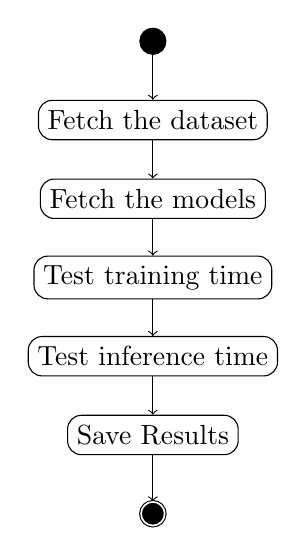
\begin{tikzpicture}
       \tikzset{start/.style ={circle,minimum width=0.3cm, minimum      height=0.3cm, draw, fill}}
       
       \tikzset{activity/.style={rectangle ,minimum width=1cm,
minimum height=0.5cm, rounded corners=5pt, draw}}

        \tikzset{end/.style={draw,double=white, circle,
                inner sep=1pt,minimum width=0.3cm,minimum height=0.3, draw, fill}}



        \node[start] (start) {};
        %\node[activity, below of = start] (action1) {Read the configuration file};
        \node[activity, below of = start] (action1) {Fetch the dataset};
        \node[activity, below of = action1] (action2) {Fetch the models};
        \node[activity, below of = action2] (action3) {Test training time};
        \node[activity, below of = action3] (action4) {Test inference time};
        \node[activity, below of = action4] (action5) {Save Results};
        \node[end,below of = action5](end){};

        \draw[->](start) -- (action1);
        \draw[->](action1) -- (action2);
        \draw[->](action2) -- (action3);
        \draw[->](action3) -- (action4);
        \draw[->](action4) -- (action5);
        \draw[->](action5) -- (end);

   \end{tikzpicture}
   \caption{Behaviour of the benchmarking suite on a conceptual level}
   \label{fig:activity_diagram_suite}
\end{figure}


The tool will allow us to study the behaviour of neural networks in order to find correlations amongst the metrics we analysed in chapter n. \ref{char_nn}, therefore the main requirement it needs to adhere to its flexibility. Applications in the field of sugar beet recognition may be subjected to various requirements and different conditions, hence the tool must be able to reflect that. In other words, it should be flexible enough so that we are able to configure it in multiple ways to reflect the various condition, but at the same time it is also able to produce results that are specific for our scope, i.e. finding the correlation between different metrics. Furthermore, we need the results to be verifiable and trustworthy. Being the foundation for further steps, we need to be able to trust the results and they need to be precise and accurate enough so that they can be reasoned about. \\
Finally, we are expecting the tool to be run on multiple devices, hence usability is also a factor to pay attention to. If the tool is too difficult to set up or run, it will lead to mismanagement of time and resources. \\
Flexibility is also a key factor for the choice of the data-set. Studies in the field of weed recognition use various techniques to collect the images for their data-sets. For example, authors of \cite{lu_survey_2020} use the BOSCH’s Bonirob system, a field robot, to collect various data about the plants, while authors of \cite{rs10111690} use Unmanned Aerial Vehicles (UAVs). Moreover, the way images are labelled is data-set dependent. 
Therefore, in order to ensure flexibility, the user must have full control over the data-set and how it is represented in the tool. \\
As already discussed in section n. \ref{sec:arch},  the choice of the architecture is limited amongst Resnet, Alexnet and VGG. The models which can be analysed will be the ones listed below. 
\begin{itemize}
\item Resnet18
\item Resnet34
\item Resnet50
\item Resnet101
\item Resnet152
\item Alexnet
\item VGG16
\item VGG19
\end{itemize}
Both the indication regarding the dataset and the choice of the models will be indicated in an external configuration file by the user. The tool will read this file before starting the test to collect the information needed to run properly. This configuration file helps to improve both flexibility and usability, in addition to automatically creating a documentation of the run for reproducibility. \\
To further increase usability, a logging system will be implemented so that information about the run and potential errors are visible to the user and can be corrected. \\

The actual implementation of the tool is done using Python and revolves around the \textit{fastai} library. This library is built on top of Pytorch, a very common library for machine learning, and offers powerful functions and high flexibility without a significant drop in performance. \cite{fastai}\\
\textit{Fastai} perfectly suits the goals of the benchmarking tool as it is \textit{''approachable and rapidly productive, while also being deeply hackable and configurable''}. \cite{fastai}\\
Thanks to \textit{fastai}, we also have the possibility to use publicly available implementations of the models listed above, hence removing possible differences in results coming from divergent implementations. 

In the following sections, we are going to describe how the training process and the inference time are analysed. 

\subsection{Analysing the Training Process}\label{sec:training_process_bench}

\begin{table}[h]
\centering
\begin{tabular}{ p{2cm} p{2cm} p{3.5cm}   }
 epoch&time&accuracy\\
 \hline
0&00:16&15.25710374116897\\
1&00:16&35.62246263027191\\
2&00:15&44.72259879112243\\
3&00:16&48.03788959980011\\
4&00:16&50.67659020423889\\
5&00:16&51.96211338043213\\
6&00:15&54.22868728637695\\
7&00:16&54.769957065582275\\
%8&00:16&55.64952492713928\\
%9&00:16&55.040597915649414\\
%10&00:16&57.408660650253296\\
%11&00:16&56.49526119232178\\
%12&00:16&58.1190824508667\\
%13&00:16&59.43843126296997\\
%14&00:16&58.15290808677673\\
%15&00:16&59.67523455619812\\
%16&00:16&58.79567265510559\\
%17&00:16&58.66035223007202\\
%18&00:16&59.81055498123169\\
%19&00:16&59.97970104217529\\
%20&00:15&60.21651029586792\\
 \hline
\end{tabular}
\caption[Example of training time results]{Example of training time results}
\label{tab:m_fast_time}
\end{table}

Training time is the primary characteristic of a model which can reveal some important information and can be used to optimise applications. 
Fastai provides 3 functions for training a model, namely \textit{fit()}, \textit{fit\_one\_cycle()} and \textit{fine\_tune()}, and each of these functions has a different purpose.\\
The function \textit{fit()} is simply a wrapper around the \textit{train()} function of PyTorch and it represents a very basic training loop. \cite{fastaidocs} \\
On the other hand, \textit{fit\_one\_cycle()} implies a phenomenon called \textit{Super-Convergence} which allows fast training of Neural Networks exploiting the learning rate. \cite{DBLP:journals/corr/abs-1708-07120}
One of the key elements of super-convergence is training with the one-cycle policy developed by \textit{Smith} in \cite{DBLP:journals/corr/abs-1803-09820}. \cite{DBLP:journals/corr/abs-1708-07120}\\
Finally \textit{fine\_tune()} can be seen as a particular combination of \textit{fit\_one\_cycle()} and \textit{(un)freeze} which works well in a lot of cases. \textit{fine\_tune()} is geared mainly towards transfer learning, i.e. towards training pre-trained models with a new dataset, since it employs the \textit{freeze()} function. Such function is used to freeze the first layers so that the weights do not get updated during further training.\cite{fastaidocs}\\
Since the three functions have different scopes and are beneficial in different kinds of applications, the benchmarking tool is configurable in a way that the preferred way of training can be chosen. \\
Once the models and the training method have been selected, the tool will start training each model accordingly for the number of epochs chosen by the user. Once the training is complete, the results are stored and then represented into a graph. \\
As suggested in section n. \ref{b_trainig_time}, there are two ways to record training time. For the purpose of this paper, we will use the first one, i.e. the one offered by \textit{fastai}. Even though the second method (Fig. \ref{fig:ben_tra}) is more precise, it does not give actual indications about the time taken for each epoch. On the other hand, this method neglects the time taken to validate the training step, hence not considering this small delay for every epoch. As a result the total training time does not comprise this delay which, even though potentially insignificant, it increases as the number of epochs increases and it will influence the total training time. However, using the first method, we also have information of the accuracy obtained at each epoch
and thus allowing us to better reason about it. Table \ref{tab:m_fast_time} shows an example of the information extracted from this process. Furthermore, this information is then extrapolated and graphed, as shown in Fig. \ref{fig:res_epo_acc} and Fig. \ref{fig:res_time_acc} and saved as a serialised file. 




\begin{figure}[th]
     \begin{subfigure}[b]{0.5\textwidth}
	    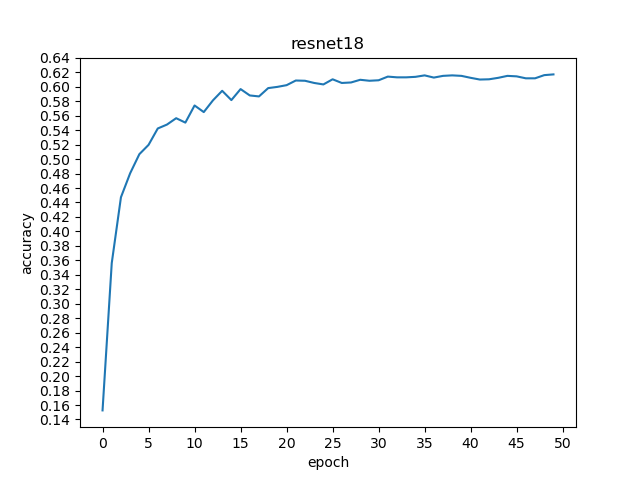
\includegraphics[width = \gw cm]{img/resnet18_epoch-accuracy.png}
	    \caption[Example of accuracy over epoch]{Example of the accuracy graphed against the number of epoch used to train for resnet18}{\centering}
	    \label{fig:res_epo_acc}
     \end{subfigure}
     \begin{subfigure}[b]{0.5\textwidth}
	    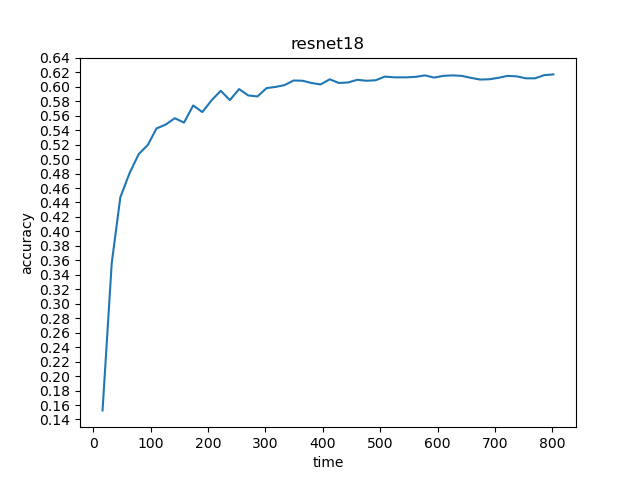
\includegraphics[width = \gw cm]{img/resnet18_time-accuracy.png}
	    \caption[Example of accuracy over time]{Example of the accuracy graphed against time taken to train in seconds for resnet18}{\centering}
	    \label{fig:res_time_acc}
     \end{subfigure}
        \caption{Example of graphs produced by the tool when analysing training time}
        \label{fig:training_time_graphs}
\end{figure}








\subsection{Analysing inference Time}
As described in section n. \ref{sec:inference_time_definition} inference time is the time needed for the model to make predictions. We discussed in section n. \ref{sec:ben_inf} different ways to measure inference time, including how to calculate it considering the architecture of the Neural Network we chose. This last method, however, is not suitable for our purpose, since it is not precise enough to lead to correct predictions, therefore the method used for the benchmark tool is the one shown in Fig. \ref{fig:corr_inf}, with the only difference that the tool will save the prediction result and calculate the total accuracy achieved. The results will be then graphed as shown in Fig.\ref{fig:infere_graph}. 
\begin{figure}[h]
\centering
	    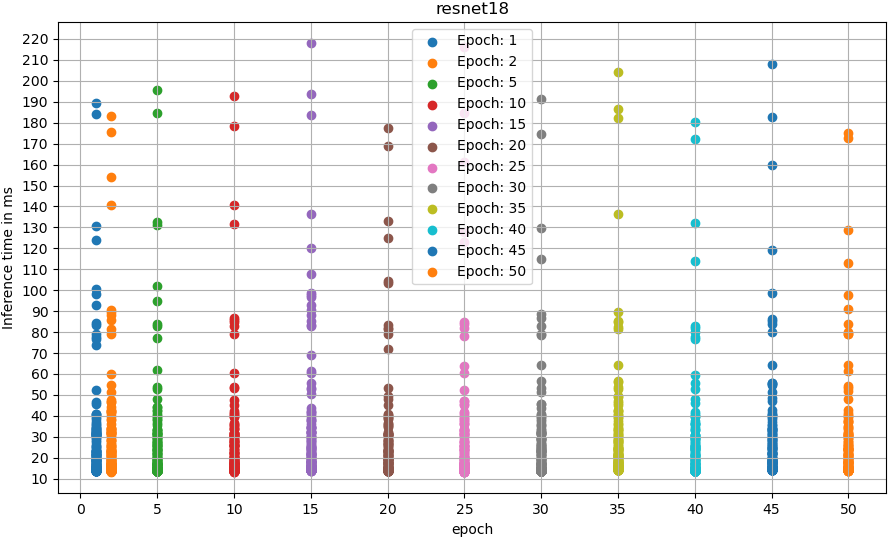
\includegraphics[width = \gw cm]{img/epoch_inferencetime.png}
        \caption{Example of the graphs produced by the tool when analysing inference time}
        \label{fig:infere_graph}
\end{figure}

Fig. \ref{fig:infere_graph} shows an example of Resnet18 trained for various epochs and tested using 50 images which were not part of the training set. 
During the analysis of inference time, the tool will calculate accuracy as the percentage of corrected predictions over the whole set, as shown in equation n. \ref{eq:cla_acc}. Since we are not going to treat any binary classification problem, we are going to avoid equation n. \ref{eq:bin_acc}. \\
Inference time is analysed based on the number of epochs used for training the models. A complete overview of the process is shown in Fig. \ref{fig:activity_diagra_inf}.\\
The user indicates a list containing all the epoch to use for training. For example, in Fig. \ref{fig:infere_graph} the epoch inserted were:
\[
1,2,5,10,15,20,25,30,35,40,45,50
\]
Once the model has been trained for the respective number of epochs and the inference has been tested, the results are saved and the model initialised. The process ends when the inference time of all the models have been trained for each epoch in the list. \\

\begin{figure}[th]
\centering
   \begin{tikzpicture}
       \tikzset{start/.style ={circle,minimum width=0.3cm, minimum      height=0.3cm, draw, fill}}
       
       \tikzset{activity/.style={rectangle ,minimum width=1cm,
minimum height=0.5cm, rounded corners=5pt, draw}}
        \tikzset{decision/.style={diamond,minimum width=1cm, minimum height=1cm, draw}}
        
        \tikzset{end/.style={draw,double=white, circle,
                inner sep=1pt,minimum width=0.3cm,minimum height=0.3, draw, fill}}



        \node[start] (start) {};
        %\node[activity, below of = start] (action1) {Read the configuration file};
        \node[activity, below =  of  start] (action1) {Fetch epochs list};
        \node[decision, below = of action1] (decision1) {done?};
        \node[activity, below =of  decision1] (action2) {next epoch};
        \node[activity, below =of  action2] (action3) {train models};
        \node[activity, below =of  action3] (action4) {test inference};
        \node[activity, below = of  action4] (action5) {save result};
        \node[activity, below = of  action5] (action6) {initialize models};
        
        \node[end, right =of  decision1] (end) {};

        
        \draw[->](start) -- (action1);
        \draw[->](action1) -- (decision1);
        \draw[->](decision1) -- (action2)node [left,midway]{no} ;
        \draw[->](action2) -- (action3);
        \draw[->](action3) -- (action4);
        \draw[->](action4) -- (action5);
        \draw[->](action5) -- (action6);
        \draw[->] (action6.west) -- ++(-40pt,0pt) |- (decision1.west);
        \draw[->](decision1) --  (end)node [above,midway]{yes};
   \end{tikzpicture}
   \caption{Overview of the process to test inference}
   \label{fig:activity_diagra_inf}
\end{figure}
\subsection{Further Analysis}
Once the tests terminate the tool stores the information collected in a file on the disk. The information stored are:
\begin{itemize}
\item Epoch
\item Training loss
\item Validation loss
\item Accuracy
\item Training time for epoch
\item Inference Time
\item Prediction
\item Ground Truth
\end{itemize}
The data, however, is serialised before being saved, therefore it can be visualised and further investigated with the use of a ready-to-use Jupyter notebook (\cite{Kluyver2016jupyter}). In addition to the raw visualisation of the data, the notebook allows the user to elaborate information for further analysis. This notebook calculates the average training time needed for each epoch, the highest accuracy achieved during training and the highest accuracy during the prediction test.  Furthermore, it also calculates precision (equation n. \ref{eq:pre}), recall (equation n. \ref{eq:rec}) and the F1-score (equation n. \ref{eq:f1_score}). \\
The notebook also gives the possibility to graph the trend of the single models during the test both over training time and epochs. In addition to the trend during training - as discussed in section n. \ref{sec:training_process_bench} - it is also possible to visualise the validation loss and training loss over training time. 
